\question{Массово-геометрические характеристики твердого тела. Моменты инерции
относительно точки, оси. Центробежные моменты инерции. Теорема
Гюйгенса-Штейнера. Вычисление моментов инерции тела относительно оси
заданного направления.}

\begin{minipage}{.38\textwidth}
    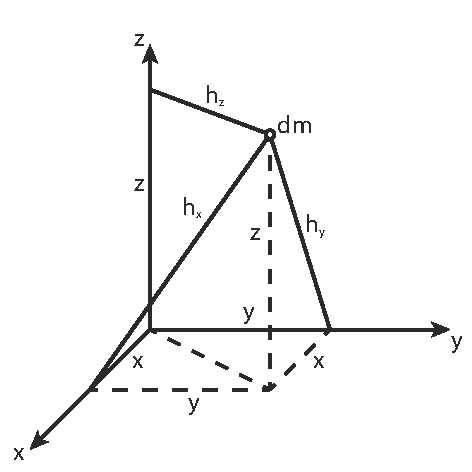
\includegraphics[width=\textwidth]{29_01}
\end{minipage} \hfill
\begin{minipage}{.57\textwidth}
    Моментом инерции материальной системы относительно оси называется сумма
    произведений масс точек системы на квадрат расстояний от точек до оси. При
    непрерывном распределении массы сумма переходит в интеграл.

    Возьмем в теле элемент с массой \( dm = \rho\,dV \) и координатами
    \( x,\ y,\ z \). Квадраты расстояний от этого элемента до координатных осей
    будут равны:
    \[
        h_x^2 = y^2 + z^2,\ h_y^2 = x^2 + z^2,\ h_z^2 = x^2 + y^2.
    \]
    
    Следовательно, моменты инерции тела относительно координатных осей равны:
\end{minipage}
\[
    I_x = \int(y^2 + z^2)\,dm, \quad I_y = \int(x^2 + z^2)\,dm, \quad
    I_z = \int(x^2 + y^2)\,dm.
\]

В этих формулах под символом интеграла подразумевается интеграл, взятый по массе
всего тела.

Центробежным моментом инерции одной материальной точки \( I_{xy} \) называется
произведение ее координат \( x,\ y \) на массу точки \( m \), то есть величина
\( xym \). Центробежными моментами инерции твердого тела называются величины,
определенные равенствами:
\[
    I_{xy} = \int xy\,dm,\quad I_{yz} = \int yz\,dm,\quad I_{zx} = \int zx\,dm.
\]
Отсюда видно, что центробежные моменты инерции симметричны относительно своих индексов:
\( I_{ij} = I_{ji} \).

\subquestion{Теорема Гюйгенса-Штейнера}
\begin{minipage}{.38\textwidth}
    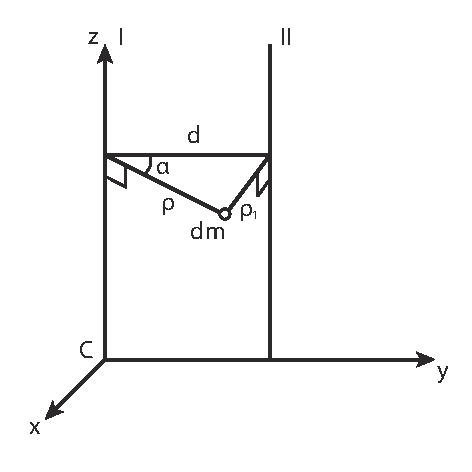
\includegraphics[width=\textwidth]{29_02}
\end{minipage} \hfill
\begin{minipage}{.57\textwidth}
    Момент инерции \( I \) тела относительно некоторой оси равен сумме момента
    инерции \( I_C \) тела относительно оси, проходящей через центр масс
    параллельно данной, и произведения массы тела на квадрат расстояния между
    осями.

    Пусть оси I и II параллельны, причем ось I проходит через центр масс \( C \)
    тела. Возьмем начало координат в точке \( C \), совместим ось \( z \) c осью
    I, а ось \( y \) направим так, чтобы она пересекала ось II. Выделим в теле
    произвольный элемент массой \( dm \) и опустим от него перпендикуляры на оси
    I и II, обозначив их соответственно через \( \rho \) и \( \rho_1 \).
\end{minipage}
Согласно определению моментов инерции, получим: \( I_C = \int \rho^2\,dm, \quad
I = \int \rho_1^2\,dm \).

По теореме косинусов получим: \( \rho_1^2 = \rho^2 + d^2 - 2\rho d\cos\alpha =
\rho^2 + d^2 - 2dy \).

Подставим это выражение в формулу, определяющую момент инерции \( I \):
\[
    I = \int (\rho^2 + d^2 - 2dy)\,dm = \int \rho^2\,dm + d^2\int dm -
    2d\int y\,dm.
\]

Первый интеграл равен \( I_C \), второй -- массе тела \( M \), а третий -- нулю.
Следовательно, \( I = I_C + Md^2 \).                                             

% было написано, что нет последней части

\newpage
